\documentclass{../src/bcthesispart}

\title{Emerging numeral systems}
\author{Bas Cornelissen}

\begin{document}

%%%%%%%%%%%%%%%%%%%%%%%%%%%%%%%%%%%%%%%%
\parttitle{Emergent numeral systems}%
	{Emergent numeral systems}
	{counting-games}{%
	% Abstract
	% --------
	}
%
%\noindent
%As Bernard Comrie once put it, numerals seem to be one of the rare cases where “present-day languages provide direct insight into the evolution of language” \parencite{Comrie2013}.
%They suggest an evolution in multiple stages, starting with words for the subitized numbers 1--4, then building up in a counting sequence, which gives rise to serialization and finally fully recursive systems that prevail nowadays.
%%In the previous chapter I discussed how three  kind of evolutionary insights they provide exactly. 
%%The reason he hints at is that restricted numeral systems presumably preceded additive and fully recursive systems.
%%All of these systems can still be found in different languages, but \emph{within} a recursive system one also finds evidence for the gradual evolution of numeral systems.
%The staged evolution was also one of the central ideas developed in James Hurford’s \emph{Language and Number}: 
%\begin{quote}
%	Numeral systems universal show marks of successive phases of invention in the building up of the whole. [...] Such universal growth marks should be accounted for in terms of historically sporadic invention and [...] the only role played by ordinary acquisition is in the relatively faithful transmission to later generations of the increments made by invention. 
%	\parencite[78]{Hurford1987}
%\end{quote}
%As a result, “one can ‘read’ the history of a system, just like the history of an old building, from the contrasting styles of its pieces, from the foundations up” (p.\ 83)
%
%\emph{Innovators} play a central role in Hurfords account of the evolution of numeral systems.
%The innovators are responsible for the invention of additive and, later, multiplicative constructions.
%After the invention of new constructions they somehow become available to the entire population.
%But given that a population can form certain constructions, the crucial question is how a linguistic innovation is eventually \emph{standardized}.
%How it can be that, roughly, \lng{three tens and two} is the standard expression for 43 and \lng{four eights} is not?
%
%Standardization can work in at least two ways: by what Hurford called \emph{diachronic elimination} and by \emph{survival-of-the-first}. 
%In diachronic elimination, a stable language community gradually decreases the range of preferred expressions for a number, until only one is left.
%The survival-of-the-first mechanism on the other hand sticks the the numerals that first appeared.
%The theory of \textcite{VonMengden2008} bears most resemblance to a survival-of-the-first mechanism.
%Indeed, if bases arise from serialized expressions that only come into use once a previously standardized counting sequence is exhausted, there never really was any room for competing expressions.
%But on the other hand, sporadic complex expressions also appear in his account before a process of serialization has even started.
%
%%
%%This explanation is somewhat problematic in the light of mixed numeral systems and ‘invasions’ of other numeral systems, and indeed Hurford gravitates towards diachronic elimination.
%%His real focus, however, is question (2). 
%%
%%
%%This is a question not addressed as such by \textcite{VonMengden2008}.
%
%
%%\textcite{Hurford1987} divides the evolution of numerals in three stages: first, a stage where a sequence of numbers for 1--10 has been standardized (phase 1 and 2 in \textcite{VonMengden2008}); second, a stage where additive constructions are standardized (phase 3); and third, a stage with multiplicative constructions (also phase 3).
%
%%From this point of view, the crucial question is how a certain 
%%Once an innovator invents new linguistic constructions, it becomes available to the entire population and do not change substantially. 
%%This is an idealization, and one might prefer to think of a phase of innovation rather than an individual innovator.
%%But in both cases, the question is how a linguistic innovation (such as additive or multiplicative constructions) is eventually \emph{standardized}.
%%How it can be that \lng{three tens and two} becomes standardized in a stable period, and \lng{four eights} does not?
%
%
%%
%%In this respect, \textcite{Hurford1987} diverges from the story outlined in the previous chapter.
%
%%
%%
%%But how can new innovations spread through a language community and become \emph{standardized}? 
%%Hurford develops several simulations aiming to show how social interactions can explain the standardization of numeral expressions.
%
%We therefore start this chapter by revisiting Hurford’s argument and the simulations on which it relies in particular.
%%After detailing his ‘reading’ of the history of numerals, the simulations are our main concern.
%I will reanalyze his results and will try to show that they do not yet explain the standardization in a satisfactory way.
%That should not be surprising, since Hurford work preceded — and importantly, anticipated — the language game simulations that attracted much attention in the nineties.
%Much of that work has centered around several \emph{Naming Games}, which I will connect to Hurfords simulations and the emergence of numeral systems.
%More concretely, I argue that a classical naming game can be used to negotiate a set of simple numerals, which fills a gap in Hurford’s account.
%This game essentially takes numbers to be unordered, directly perceivable quantities and corresponds to what Hurford called the \emph{referential-pragmatic} account of numbers.
%I then propose and analyse (three variants of) a new naming game, the \emph{Counting Game} in which a population of agents negotiates a sequence of words.
%This sequence functions as a counting sequence and thus corresponds to two different conceptions of numbers: the \emph{conceptual-verbal} and \emph{ritual} view.
%
%
%

\section{Standardizing a base}

%According to \textcite{Hurford1987}, cultural evolution left growth marks on numeral systems.
%First, the numerals up to 3--4 tend to behave differently. 
%Then, numbers up to the first base mostly have monomorphic expressions.
%Between the first base and its first multiple (e.g.\ between 10 and 20) the syntax often suggests additive constructions, as seen from for example 1-deletion. 
%Multiplicative constructions presumably arised only later. 
%As a result, the base is often expressed using a variety of phonological forms (base-suppletion).
%This suggests roughly that the cultural evolution of numeral systems can be divided in roughly three stages: a first stage where only simple numerals are used, a second stage with additive constructions and a third stage with multiplicative constructions.


%As said, \textcite{Hurford1987} attributes transitions between these stages to linguistic innovators.
%These innovators occasionally invent new linguistic constructions or, in our case, ways to generate new numerals. 
%Between phases of linguistic innovation the rules become available to the entire population and do not change substantially. 
%This is an idealization, and one might prefer to think of a phase of innovation rather than an individual innovator.
%But in both cases, the question is how a linguistic innovation (such as additive or multiplicative constructions) is eventually \emph{standardized}.
%How it can be that \lng{three tens and two} becomes standardized in a stable period, and \lng{four eights} does not?
%
%Hurford divides the question of the standardization of numerals in two subquestions: (1) why and how does standardization of numerals occur at all, and (2) given that it happens, why does it take the form it in fact does?
%Standardization can work in at least two ways: by \emph{diachronic elimination} and by \emph{survival-of-the-first}. 
%In diachronic elimination, a stable language community gradually decreases the range of preferred expressions for a number, until only one is left.
%The survival-of-the-first mechanism on the other hand sticks the the numerals that first appeared.
%This explanation is somewhat problematic in the light of mixed numeral systems and ‘invasions’ of other numeral systems, and indeed Hurford gravitates towards diachronic elimination.
%His real focus, however, is question (2). 



%%%%%%%%%%%%%%%%%%%%%%%%%%%%
% SUBSECTION
\subsection{The Additive and Multiplicative Base Game}
Why does a particular base, such as 10, emerge as the standard base in a community? 
Hurfords (1987) answer takes the form of two simulations in which populations of simple agents negotiate a decimal system.
Simulations of this kind are nowadays usually called ‘games’ and for that reason I have baptised Hurfords simulations the \emph{Additive} and \emph{multiplicative Base Game} (\textsc{bg}).
%Since the original analyses were fairly informal, 
I will start by reanalyzing both.



In both games, populations of $N$ agents “spend their time uttering numeral expressions to each other”.
Interaction between agents are assumed to be (uniformly) random and homogeneous: any two agents can interact.
In every encounter, a speaker utters an expression to a hearer: constructions like $7+6$ or $3\times 10 + 5$.
Initially, all agents will use different expressions for the same numbers, but over time the same \emph{base} should be used to form expressions.
As we have seen, a base is only defined inside a numeral system.
What then, would be the base of an expression before a system has even emerged?
In additive expressions $x+y$, Hurford takes the base to be the largest of the constituents, $b=\max(x,y)$ whereas in multiplicative constructions $x\times y + z$, the base is the largest of the factors $b = \max(x,y)$.
So $3\times 7, \;\; 4 \times 7 + 3$ and $4+7$ all use base 7. 
This definition is not unproblematic, but let’s see how far it goes.



We assume speakers try to use expressions that a hearer is likely to know.
To that end agents track the frequencies $f(b)$ of all bases $b$ they encounter and use bases that they have seen frequently.
A simple criterion decides which bases are \emph{favoured}, i.e.\ which bases an agent prefers to use.%
	\footnote{The criterion differs from Hurfords criterion in that I require $f(b)>0$. 
	This additional requirement does not change the behaviour of the game: if no bases are favoured, agents also have to make a random choice from all bases. 
	It does, however, align the reported quantities with games encountered later on.}
A base $b$ is \emph{favoured} if 
	\begin{align}\label{eq:favoured-base-criterion}
		f(b) > 0 \qquad \text{and} \qquad f(b) \ge \frac{1}{\eta} \cdot \max_{b'} f(b'),
	\end{align}
for some $\eta>1$.
The criterion is less restrictive for larger $\eta$ as it lowers the threshold for being favoured.
In the extreme case $\eta=1$, favoured bases are those with positive and \emph{maximal} frequency.



\paragraph{additive base game}
The \emph{Additive Base Game} models a population in the second stage of Hurfords account of the evolution.
That is, all agents know simple numerals for $1, \dots, 10$ and moreover know how to combine them to form additive constructions.
They can thus express the numbers 1 to 20 with expressions of the form $6+7$ and $10+5$.
Not every number is equally ‘useful’ for expressing higher numbers using only addition.
10 is most useful, as you can express any number between 11 and 20 as $10 + n$, $1\le n \le 10$. 
With 9 you can only get to 18, with 8 up to 16, and so on. 
\textcite{Hurford1987} argued that as a result of this, 10 will soon become the most frequent base.
Over time the expressions $10+1, 10+2, \dots, 10+10$ become standardized and the population eventually adopts a decimal system.
The game was proposed to test the consistency of this account and follows the following script.
\begin{enumerate}
	\item A number $n$ is chosen from a set of numbers $\mathcal{N} = \{11, \dots, 20\}$.

	\item The speaker $S$ finds an expression for $n$. 
		\begin{enumerate}
			\item To that end, the speaker considers a set $C$ of candidate bases: favoured bases which can be used to express $n$, that is, for which $n \le 2b$.
				So if $n=17$ and 7 and 9 are the favoured bases, then $C = \{9\}$ since only base 9 can express 17 (as $9+8$).
			\item If $C$ is not empty, the speaker randomly picks a base $b$ from $C$; otherwise she randomly picks one of the bases that \emph{would} express $n$.
			\item $S$ expresses $n$ as $b + (n-b)$.
		\end{enumerate} 
		
	\item The hearer $H$ receives the expression $e$. After determining the base $b$ used, $H$ updates the frequency $f_H(b)$ of $b$ by 1.
\end{enumerate}




\paragraph{multiplicative base game}
The second game, the \emph{Multiplicative Base Game}, corresponds to the third stage in the evolution of numeral systems, after an innovator has invented multiplicative constructions of the form $f\times b +r$.
As before, agents track base-frequencies to determine which they favour. 
But there is an additional criterium. 
If an agent favours several bases it can express certain numbers in multiple ways.
For example, if 10, 9, 8 and 7 are all favoured, 21 can be expressed as
$\;2\times 10 + 1$, \; $2\times 9 + 3$,\; $2\times 8 + 5\;$ and $\;3 \times 7$.
In this case agents prefer \emph{simpler} expressions --- here $3 \times 7$ --- as the result of a general simplicity bias \parencite{Hurford1987}.
Step 2 of the script is changed slightly to accommodate this:
\begin{enumerate}\setcounter{enumi}{1}
	\item The speaker $S$ finds an expression for $n$. 
	\begin{enumerate}
		\item As before consider the candidates $C$: favoured bases $b$ which can be used to express $n$, that is, $b$’s for which $b \le n \le b^2+10$.
		\item Pick a random base $b$ from $C$ or, if it is empty, use a random other base that can express $n$.
		\item Consider all decompositions $n=f\times b + r$. If there are simple decompositions $n=f\times b$ communicate one of those, otherwise communicate a random other expression.
	\end{enumerate} 
\end{enumerate}
Note that the remainder can thus be larger than the base.



\subsection{Basic Phenomenology}
The dynamics of the games can be studied by collecting several  statistics \parencite[cf.][]{Baronchelli2017,Wellens2012}, typically with a certain resolution (e.g.\ after every 10 time steps).

\begin{itemize}
	\item \textbf{(Probability of) communicative success $p_s(t)$} The probability that an interaction at time $t$ is succesfull. We consider an interaction successful if the base used by the speaker is favoured by the hearer. We estimate the probabilities by averaging this binary variable over many runs.
	\item \textbf{Base count $N_{\text{base}}(b, t)$.} 
		The number of agents that favour base $b$ at time $t$.
	\item \textbf{Total base count $N_{\text{total}}(t)$} 
		The total number of bases favoured by agents in the population.
		It can be computed as the sum of the base frequencies:\
		\[ 
			N_{\text{total}}(t) = \sum_b N_{\text{base}}(b, t).
		\] 
		When divided by the population size $N_{\text{total}}(t)/N$ gives the average number of bases favoured by agents at time $t$.
	\item \textbf{Unique base count $N_{\text{unique}}(t)$.} The number of unique bases favoured in the population at time $t$. This, too, can be computed from $N_{\text{base}}(b, t)$ as
		\[
			N_{\text{unique}}(t) = |\{b: N_{\text{base}}(b, t) > 0\}|.
		\]
\end{itemize}
Due to the stochasticity of the games, individual runs vary substantially and often obscure underlying regularities.
Conversely, the behaviour of a single run can also suggest regularities that do not generalise.
It is therefore more informative to study the average behaviour of the games by running simulations several times and averaging the listed statistics over all runs.

\begin{SCfigure}
	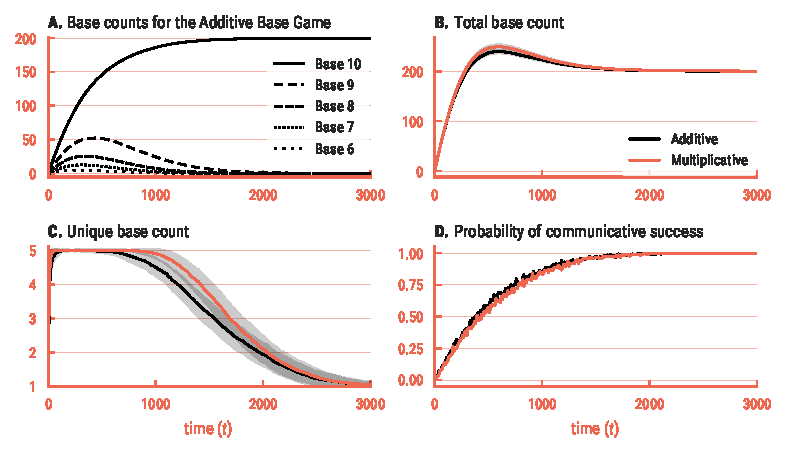
\includegraphics[trim=\figleftmarginA{} 0 0 \figtopmargin]{HUR03-results}	
	\caption{Comparison between the Additive Base Game (black) and the Multiplicative Base Game (orange). 
		The dynamics of the two games are remarkably similar.
		Dynamics are visualized using
		\subfig{A} the base counts of all possible bases for the Additive Base Game only (the Multiplicative case looks extremely similar);
		\subfig{B} the total base counts;
		\subfig{C} the unique base count; and
		\subfig{D} the probability of successful communication.
		See main text for details.
		\\[1em]
		Results shown for $N=200$, $B=10$; avg.\ of 600 runs; 1 std.\ shaded.
		\label{fig:add-vs-mul}}
\end{SCfigure}

Figure \ref{fig:add-vs-mul} summarizes these average statistics, obtained from 600 runs of the additive and multiplicative \textsc{bg} in populations of $N=200$ agents.\footnote{I have tried to be consistent in the choice of parameters in different simulations. I will therefore not repeat them in the main text and instead list them in the captions of the relevant figures.}
Subfigure A illustrates the typical stages every simulation goes through.
Initially, none of the bases is favoured and bases are used with roughly equal probability.
This is followed by a phase in which different bases compete for a share of the population.
The largest two bases are, initially, the two biggest competitors, but one of them (10) soon takes over, leading to the emergence of a shared numeral system.
The same behaviour can also be illustrated in the other subplots B--D. 
From B one can clearly see that the total number of bases favoured by agents crosses the population size $N=200$, indicating that at the peak multiple bases compete for each agents preference.
Plot C clearly illustrates that it takes a long time to eliminate all other bases from the population, even if base 10 is already odominant.
Finally, in D one sees that interactions become more and more successful as the population settles on one numeral system.


In short, the local interactions between the agents are enough to establish a global consensus in the form of a shared numeral system.
%In short, the simulations support the idea that local interactions alone can lead to a global consensus: a shared numeral system.
Moreover, Hurfords intuition that a decimal system would be adopted is confirmed.
Do these simulations provide a good account of the emergence of a decimal system? 
Answering that will require further analyses. 
First we need to clarify how the parameters influence the games.
Since the behaviour of the two games is so comparable, I will not repeat all analyses for both games.


\paragraph{Effect of $\eta$}
Recall that the parameter $\eta$ determined which bases were favoured (see equation \ref{eq:favoured-base-criterion}).
The additive \textsc{bg} was repeatedly simulated for $\eta \in \{1, 2, 3\}$ and the results are reported in figure \ref{fig:effects-eta}.
Higher values of $\eta$ slow down convergence and increase the variance across runs. 
This is not surprising: when $\eta=3$, an agent only favours a single base if its frequency is 3 times as high as that of any other base. 
Since the behaviour seems otherwise comparable, I have used $\eta=1$ throughout. This means that agents favour bases with \emph{maximal frequency}.

\begin{SCfigure}
	%% RESULTS HUR02
	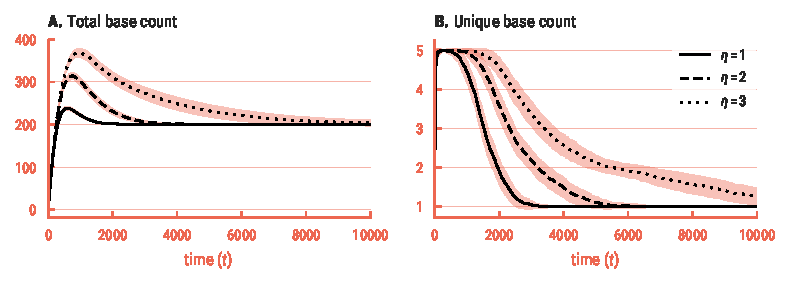
\includegraphics[trim=\figleftmarginA{} 0 0 \figtopmargin]{HUR02-results}	
	\caption{Effects of $\eta$, the parameter that determines which bases are favoured, in the \textsc{abg}. 
		Dynamics are visualized using
		\subfig{A} the total base count and
		\subfig{B} the unique base count.
		$\eta$ strongly influenes the convergence time.
		\\[1em]
		Results shown for $N=200$, $B=10$; avg.\ of 300 runs; 1 std.\ shaded.
		\label{fig:effects-eta}}
\end{SCfigure}

\begin{SCfigure}
	% Results HUR01b
	\includegraphics[trim=\figleftmarginA{} 0 0 \figtopmargin]{HUR01b-results}	
	\caption{The effect of $B$, the number of simple numerals, in the \textsc{abg}. One effect is \emph{not} shown: the population always adopte $B$ as a base (see main text for details).
		\\[1em]
		Results shown for $N=200$, $\eta=1$; avg.\ of 300 runs; 1 std.\ shaded.
		\label{fig:effect-B}}
\end{SCfigure}

\paragraph{effects of the number of simple numerals}
How does the number of simple numerals influence the game?
To find out, we reformulate the games in more general terms.
Let us say that agents have simple numerals for the numbers 1 to $B$ (where previously $B=10$). 
This allows for additive constructions from $B+1$ to $B+B$ (11 to 20) and multiplicative constructions from $B+1$ up to $B^2+B$ (11 to 110). 
Possible bases lie between $b_0=\text{ceil}(B/2)$ and $B$ (6 and 10).
The Additive Base Game has been simulated for $B\in \{5, 10, \dots, 30\}$ and the resulting dynamics are shown in figure \ref{fig:effect-B}. 
Several things should be noted. First, the convergence time does not seem to be affected by $B$.
Second, and this cannot be seen from figure \ref{fig:effect-B}, the population adopts a different base when more simple numerals are available. 
%--> See experiment HUR01a
More precisely, the population consistently adopted the highest possible base, which is $B$.




\subsection{Further analyses}
What do the simulations tell about the standardization of numeral bases?
As said, it shows that standardization does not require centralized coordination.
In the next section we will see that this is a general property of these types of language games.
First we ask: why exactly does the population adopt a decimal system?


\begin{SCfigure}
	% Results HUR05
	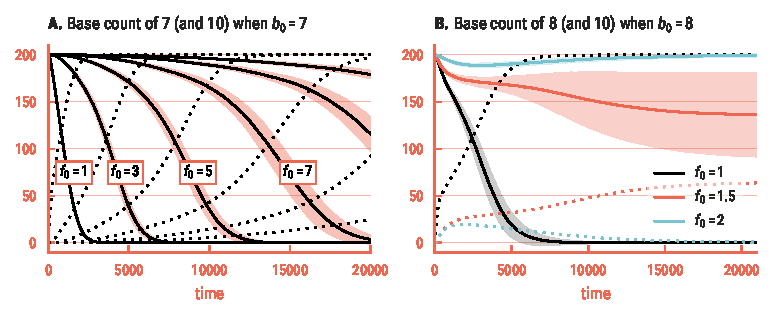
\includegraphics[trim=\figleftmarginA{} 0 0 \figtopmargin]{HUR05-results}	
	\caption{The effects of initial conditions in the \textsc{abg}. Every agent initially assigns frequency $f_0$ to base $b_0$ which in some cases prevents the population from converging to a decimal system.
		The plots illustrate markedly different behaviour in populations biased towards base 7 or base 8.
		\subfig{A} Base counts when $b_0=7$ and $f_0 \in \{1, 3, 5, 7, 9\}$ (annotated). The counts of base 10 are also shown (dotted). 
		\subfig{B} Similar, but $b_0=8$ and $f_0 \in \{1, 1.5,2\}$.
			Note that the results averages over 300 simulation runs, so for $f_0=1.5$ different runs convert to either base 10 or base 8.
		\\[1em]
		Results shown for $N=200$, $\eta=1$, $n_{\text{max}}=46$; avg.\ of 300 runs, 1 std.\ shaded.
		\label{fig:effect-initial-conditions}}
\end{SCfigure}



\paragraph{initial conditions}
Hurford argued that this was a result of the domain about which the agents had to communicate.
When agents communicate about $n_{\text{min}}=11$ to $n_{\text{max}} = 110$, then base 10 has an advantage since it is the only one that can be used to express all these numbers. 
This expressive advantage, Hurford suggests, will quickly make $10$ the most frequent base, resulting in a decimal system. 
We have seen that for values of $B$ other than 10, the population also adopts a base-$B$ system, which supports Hurford's account. 
However, it cannot be entirely accurate, since we can find strong effects of initial conditions.
Consider a biased population where every agent initially assigns a frequency $f_0$ to one particular base $b_0$.
All agents thus appear to have encountered $f_0$ uses of $b_0$.
The above account suggests that the situation will be unstable if $b_0\neq 10$. That is, if $b_0<10$, the population will over time stop using $b_0$ and switch to a decimal system instead. 



Figure \ref{fig:effect-initial-conditions} reports the results of two experiments with the multiplicative \textsc{bg} that show this is not the case.
The first experiment used initial base $b_0 = 7$ and various initial frequencies $f_0 \in \{ 1, 3, 5, 7, 9\}$.
The time to convergence clearly increases with $f_0$, but eventually base 10 will take over.
Base 7 thus appears to be unstable.
The case for base 8 is quite different, as shown by the second experiment, with $b_0 = 8$ and $f_0 \in \{1, 1.5, 2\}$. 
As figure \ref{fig:effect-initial-conditions} illustrates, base 8 is unstable for $f_0=1$, but stable for $f_0=2$, despite its expressive disadvantage.
I have included $f_0 = 1.5$ to illustrate the effects of an bias of intermediate strength (one might think of it as biasing half the population with $f_0=2$).
Note that the plots are averaged over 300 runs, so at $t=20\; 000$ half of the runs had adopted a base-8 system, and in the remaining runs a based-10 system.
The results point to a bifurcation between $f_0=1$ and $f_0=2$ (and $b_0 = 7$ and $b_0 = 10$), where base $8$ changes from being unstable to being stable.
In short, other bases than 10 can be stable, given the right initial conditions.
These experiments also show that the multiplicative \textsc{bg} captures two mechanisms of standardization: both survival-of-the-first \emph{and} diachronic elimination.





\paragraph{domain adaptivity}
Returning to the original question, did the decimal system emerge because of an expressive advantage \emph{and} the right initial conditions? 
Even this answer is not entirely accurate.
%So the original question is still open: why the decimal system?
%So far, it appears to emerge because it has an expressive advantage.
%As an aside, neither is it a very plausible explanation for the structure of numeral systems.
%First of all, because it predicts that higher bases are more likely to be adopted, while in fact bases higher than 20 are rare.
%Second, systems use multiple bases to counter expressive restrictions.
%The disadvantage of a sextary system in the games is in reality for example ameliorated by introducing the larger base 36.
To find out why, one has to ask which base, if any, is standardized if \emph{none has an expressive advantage}. 
%One way to do so is by following common practice and extend the game with higher bases.
%However, one might argue that this gives larger bases a different advantage: a decimal system needs fewer bases to express the numbers up to 100 than a sextary system.
%But conversely, using higher bases require longer sequences of simple numerals (ignoring additive bases). 
%If and how such a trade-off could work out might be an interesting question in itself,%
%	\footnote{One wonders, for example, if it could be the case that typical bases best accommodate the range of numbers that needs to be expressed most often --- if such a range exists independently of the spoken language at all.} 
%	but can also be sidestepped.
A simple way to ensure that all bases have equal expressive power is by restricting the range of communicated numbers to the range expressible with the smallest base.
Using the above notation, that means asking agents to communicate up to $n_{\text{max}} = b_0\times b_0 + B$, that is, 46.



\begin{SCfigure}
	% Results HUR05
	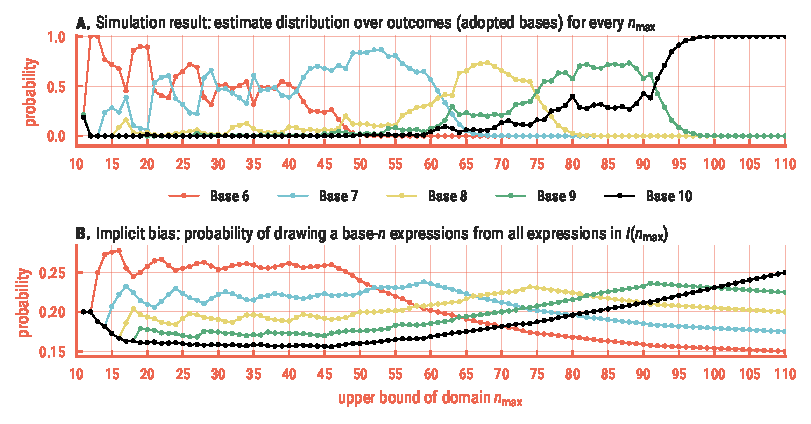
\includegraphics[trim=\figleftmarginA{} 0 0 \figtopmargin]{HUR07-results}	
	\caption{ASDFsd
		\\[1em]
		Results shown for $N=200$, $\eta=1$; avg.\ of 150 runs, 1 std.\ shaded.
		\label{fig:effect-n-max}}
\end{SCfigure}

The next experiments does that, and more.
It aims to identify to which bases the population converges if the domain is restricted to $[11, n_{\text{max}}]$ with $n_{\text{max}} \in \{11, 110\}$.
In different runs different bases might appear, so we hope to find an informative distribution over bases for every $n_{\text{max}}$ by averaging over 150 runs.
Figure \ref{fig:effect-n-max}A visualizes those distributions.
Above every point on the $x$-axis, a distribution over bases is plotted, both as points indicating their individual probabilities and as probability sticks in the background.
What it clearly shows is that every base dominates on a part of the domain. 
When agents communicate about $[11,21]$, base $6$ is adopted most frequently, when communicating about $[11,70]$, $8$ is most likely to emerge, etc.
The pattern is not particularly smooth, partly because every distribution is estimated from only 150 points.
But there might be a structural reason for the jumpiness.

How many ways are there to express a number $n$ using base $b$?
Consider $n=26$ and $b=6$.
The only possible expressions are $4 \times 6 +2$ and $3\times 6 + 8$. 
More generally, the only two base $b$-expressions are of the same form:
\[
	x\times b+r \quad \text{and} \quad (x-1) \times b + (b+r).
\]
After all, for any lower factor $x-2$, the remainder would be at least $b+b+r > 2b > B$, and therefore inexpressible. 
There is simply no simple numeral for it — that's how the game works.
Now we also see how many base-$b$ expressions a number $n$ has: none if $n > b^2+B$; one if $b+r > B$ or $r = 0$ since preference is given to the the simpler $x\times b + 0$; and two otherwise. 
As an exercise in visual mathematics, figure \ref{fig:num-expr-per-base} show for every base how many expressions there of every number in $[11, 111]$. 
You can clearly see there that for lower numbers, base $6$ has more expressions than base $10$. 

\begin{SCfigure}
	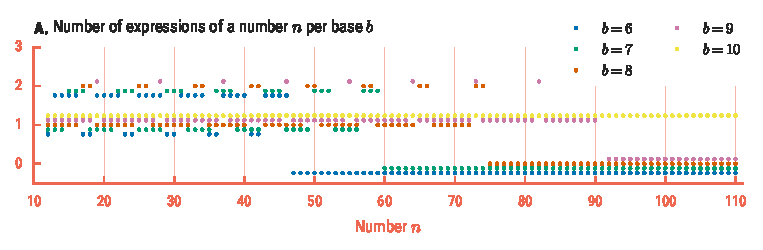
\includegraphics[trim=0.51cm 0 0 \figtopmargin]{HUR07b-results.pdf}
	\caption{The number of expressions of a number $n$ per base $b$.
	\label{fig:num-expr-per-base}}
\end{SCfigure}

That intuition underlies figure \ref{fig:effect-n-max}B.
It shows the probability of drawing an expression using base $b$ uniformly from all expressions for numbers in the interval $[11, b_{\text{max}}]$, for every $n_{\text{max}}$. Formally, let $E(b, n_{\text{max}})$ be the total number of expressions for numbers in the interval $[11, n_{\text{max}}]$ using base $b$, then the figure shows 
	\[ 
		p(b \mid n_{\text{max}}) = \frac{E(b, n_{\text{max}})}{\sum_b E(b, n_{\text{max}})}
	\] 
	for every $b$ and $n_{\text{max}}$.
In terms of the game, consider an agent that is favouring all bases.
When expressing a number, the probability of using a particular base is not uniform — it follows the distribution shown in figure \ref{fig:effect-n-max}B.
So for low $n_{\text{max}}$ using base 6 is slightly more likely and as $n_{\text{max}}$ grows, 7 becomes more likely, then 8, 9 and finally only 10.
This clearly does not yet explain the rough pattern in figure \ref{fig:effect-n-max}A, but the qualitative correspondence does suggest that the population is doing some kind of frequency matching or amplification.
The structure of the numbers is such that the pattern becomes somewhat eccentric.



%All this has little bearing on numeral systems. 
%As I have argued already, domain limitations are not a particularly strong explanation for the adoption of a certain base.
%Moreover, the fact that base 6 can on average express low numbers in more ways than base 10 can, is only because the game allows the remainder to be larger than the base. 
%Such overrunning is, as we have seen, rarely found in actual numeral systems.
%Despite these reservations, the experiments do clearly illustrate that simple language games can exhibit complex dynamics as a result of the structure of the underlying domain.


\subsection{Conclusions}
What does all this tell us about numeral systems?
Most importantly, they corroborate the idea that social interactions can lead to the standardization of a base.
But when asking \emph{why} the standardization take place, the mechanism appears to be highly problematic.
The last experiments suggest that the additive and multiplicative \textsc{bg} match or amplify the frequencies of bases in expressions of numbers in a certain domain.
Depending on both the initial conditions and the communication domain, these frequencies vary and thus change the emerging base.


Clearly, domain adaptivity is not a very plausible explanation for the structure of numeral systems.
First of all, because it predicts that higher bases are more likely to be adopted, while in fact bases higher than 20 are rare.
Second, systems use multiple bases to counter expressive restrictions.
The disadvantage of a sextary system in the games is in reality for example ameliorated by introducing the larger base 36.
Moreover, the fact that base 6 can on average express low numbers in more ways than base 10 can, is only because the game allows the remainder to be larger than the base. 
Such overrunning is, as we have seen, rarely found in actual numeral systems.
In that respect, the eccentric domain effects illustrated in figure \ref{fig:effect-n-max} are really an artefact of allowing remainders to be larger than the base.

\textcite{Hurford1987} introduced the two games partly as an explanation of the packing strategy.
On the largest domain $n_{\text{max}} = 110$ the packing strategy is indeed respected, but if the domain is a little restricted it is violated.
In a population adopting a base-6 system, both the expressions $3\times 6 + 8$ and $4 \times 6 + 2$ would be in use. 
The former would violate the packing strategy. 
It should furthermore be noted that the population has not uniquely standardized expressions; some (reduced) synonymy remains present.
This, too, is an artefact of overrunning remainders.

\mcomment{Should I check what happens if you don’t have overrunning remainders? Would make a lot of sense. But also a lot of extra work...}

Finally I would like to comment on some ‘failed’ experiments, where I accidentally took the base to be the largest of \emph{all} constituents and moreover allowed factors to be larger than bases.
If such agents communicated about the a domain expressible by all bases, the emergent base would \emph{not} tend to be the smallest base.
Instead, they would tend to adopt bases in the order corresponding to the ordering of  $p(b \mid n_{\text{max}} = 46)$ in those games.
In this case, the most frequent base was the \emph{largest prime base}.
It appeared to be the result of the simplicity bias, since when removed, the likelihood of different bases followed their natural order.
The first reason I mention this is that in all cases, $p(b \mid n_{\text{max}} = 46)$ (computed for that particular, wrong scenario) appeared a fair predictor of the probability that a base would be adopted.
This corroborates the idea that population is essentially amplifying frequencies.
The second reason is that it is striking that these games so easily pick up on the structure and limitations of the underlying domain, resulting in fairly complex behaviour.
In the case of numeral systems, that behaviour might be unrealistic, but more plausible behaviour might emerge in other domains (e.g.~colour terms).











\section{Naming Games}
To overcome some of the problematic conclusions from the additive and multiplicative naming game, it will be helpful to consider more recent work on language games.
James Hurford was after all pioneering the use computer simulations as a way of testing linguistic hypotheses.
It was only a decade later when work in this field started making substantial progress.
Around 1996, Luc Steels worked on the models than happen to be closely related to Hurfords simulations.
Those language games form the core of the remainder of this chapter.
They have been intensely studied, especially after one of them, the \emph{Naming Game}, attracted the attention of statistical physicists, most notably Andrea Baronchelli.
I will summarize some important results in this tradition
%%, largely following the presentation of \textcite[][ch.\ 2]{Wellens2012}, 
and then connect it to Hurfords work and the emergence of numeral systems.
We start with the simplest language game.


%James Hurford was one of the first to use computer simulations as a way of testing linguistic hypotheses. 
%Nearly ten years later, \textcite{Kirby1996} would still consider the simulation methodology “fairly unusual” in linguistics (p.\ 32) and only managed to find a handful of precedents.
%But another ten years later the situation had radically changed.
%Since 1996 both Kirby and Luc Steels started a line of linguistic research that heavily relied on simulations. 
%Simon Kirby, a student of Hurford, developed the \emph{Iterated Learning framework} which we will consider in the next chapter. 
%Luc Steels at the same time worked on the models than happen to be closely related to Hurfords simulations.
%Those language games form the core of the remainder of this chapter.
%They have been intensely studied, especially after one of them, the \emph{Naming Game}, attracted the attention of statistical physicists, most notably Andrea Baronchelli (2006 — indeed, another ten years later)\nocite{Baronchelli2006}.
%I will summarize some important results in this tradition
%%, largely following the presentation of \textcite[][ch.\ 2]{Wellens2012}, 
%and then connect it to Hurfords work and the emergence of numeral systems.


%\subsection{Naming games}

%\paragraph{the minimal naming game}
%The simplest is arguably the \emph{Minimal Naming Game} \parencite{Baronchelli2006,Baronchelli2017}.
%Picture a group of people encountering a colourless green object for which they do not have a name. 
%Of even worse, suppose they don’t have a shared language at all.
%Confused, I suppose, they furiously start inventing and shouting out names for the object.
%And gradually, by carefully attending to what the others are saying, they align their vocabularies, until they have agreed on a word for the object — \emph{gavagai}, perhaps. Or \emph{covfefe}.
% 
%%todo: present for multiple objects, following Wellens formalism.
%%todo: explain that this is the same as a single object, multiple times.
% 
%As before, it all starts with a population of $N$ agents.
%Each keeps an initially empty inventory of words, its \emph{vocabulary}.
%In every ‘round’, two random agents interact. 
%The speaker chooses a random word from her vocabulary, or cooks up a new word if it is empty, and communicates this to the hearer. 
%Now two things can happen. 
%Either the hearer knows the word and the communication is successful, or she does not know the word and communication fails.
%On successful communication, both agents forget all words except the successfully communicated word.
%If communication fails, the hearer ‘learns’ the word, that is, adds it to her vocabulary. This is illustrated in figure \ref{fig:minimal-naming-game-updates}.
%
%\begin{SCfigure}\sffamily\footnotesize\color{main}
%	\begin{tabular}{@{}lllll@{}}
%		\multicolumn{5}{@{}l@{}}{\color{black}\textbf{A.} Failed communication}\\\toprule
%		\textsc{speaker}	& \textsc{hearer} 
%			&$\Longrightarrow$ &\textsc{speaker}		& \textsc{hearer}
%		\\\cmidrule{1-2}\cmidrule{4-5}
%		\textbf{Gavagai}	& Spam 
%			&&\textbf{Gavagai}	& Spam\\
%		Cofveve				& Foo
%			&&Cofveve			& Foo\\
%		Spam				&
%			&&Spam				&\textbf{Gavagai}\\
%		\cmidrule{1-2}\cmidrule{4-5}
%	\end{tabular}
%	\hfill
%	\begin{tabular}{@{}lllll@{}}
%		\multicolumn{5}{@{}l@{}}{\color{black}\textbf{B.} Successful communication}\\\toprule
%		\textsc{speaker}	& \textsc{hearer} 
%			&$\Longrightarrow$ &\textsc{speaker}		& \textsc{hearer}
%		\\\cmidrule{1-2}\cmidrule{4-5}
%		Gavagai		& \textbf{Spam} 
%			&&\textbf{Spam}	& \textbf{Spam}\\
%		Cofveve				& Foo &&&\\
%		\textbf{Spam}		&&&\\
%		\cmidrule{1-2}\cmidrule{4-5}
%	\end{tabular}
%	\caption{The updates of the Minimal Naming Game illustrated. 
%		If communication fails, the hearer adss the word uttered by the speaker (bold) to its vocabularies. 
%		If it successfull, however, both empty their vocabularies and keep only the communicated word. \label{fig:minimal-naming-game-updates}}
%\end{SCfigure}
%
%
%\begin{SCfigure}
%	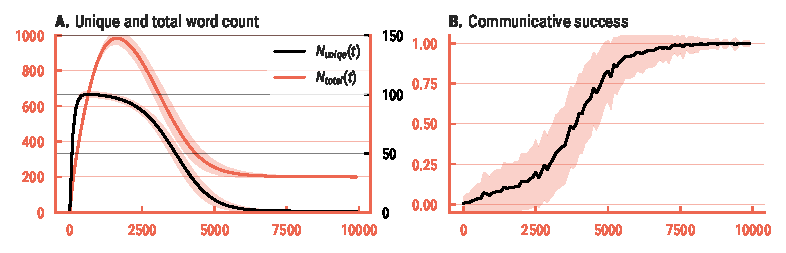
\includegraphics[trim=0.94cm 0 0 \figtopmargin]{MNG01-results}
%	\caption{The dynamics of the minimal naming game.
%		An sharp transition leads to convergence and the emergence of consensus.
%		\\[1em]
%		Results shown for $N=200$; avg.\ of 300 runs, 1 std.\ shaded.
%		\label{fig:minimal-naming-game}}
%\end{SCfigure}
%
%
%
%Interestingly, this game always has the same time dynamics, which is illustrated in figure \ref{fig:minimal-naming-game}. 
%%The quantities plotted there are analogous to those used above: $N_{\text{unique}}(t)$ is the unique word count at time $t$, $N_{\text{total}}(t)$ the total word count, and $$
%In the first phase, most interacting agents will have empty vocabularies and thus invent new words. This results in a sharp increase of the number of unique words $N_{\text{unique}}(t)$ in the population, only to stabilizes at on average $N/2$ unique words not so much later.
%As the vocabularies of agents still hardly overlap, words will rarely be eliminated --- that only happens after successful interactions.
%The total number of words $N_{\text{total}}(t)$ known by agents in the population will thus continue to grow after a bit longer, even if $N_{\text{unique}}(t)$ has already stabilized. 
%When communications start to be successful, the vocabularies however start to shrink, and $N_{\text{unique}}(t)$ declines until the entire population settled on a vocabulary with the same word.
%
%%
%%The Minimal Naming Game can also be used to negotiate multiple words. 
%%Suppose there are multiple objects $o_i \in \mathcal O$ and every round starts with the speaker picking one of the objects (the topic) and uttering a name for it. 
%%Then the hearer interprets the name and points to the specific object. 
%%Now suppose that no word ever names two objects, that is, suppose there is no homonymy. 
%%Then every round is identical to a round in the single-object version, since there can be no ambiguity about the topic.
%%In the absence of homonymy, the multi-object naming game becomes a mix of single-object naming games.
%%Therefore it 
%
%Many of the questions statistical physicists raised, concerned \emph{scaling} relations: how certain quantities scale with the size of the system \parencite{Baronchelli2017}.
%Although interesting, connecting these findings to actual language can be problematic%
%	\footnote{Baronchelli for example found that “the cognitive effort an agent has to take, in terms of maximum inventory size, \emph{depends on the system size} and, in particular, diverges as the population gets larger” \parencite[][italics in original]{Baronchelli2017}.
%	I would be hesitant to concede that linguistic activity in a small language community requires less cognitive effort than the same activity in a larger community.}
%	 and I will therefore not systematically investigate such questions.
%Nor will I investigate effects of network structure.
%Briefly, when agents are organized in a social network and only connected agents can interact, the topology of the network has been found to strongly influence the dynamics of the game \parencite{Baronchelli2017}.
%Here, I only consider the case when \emph{all} pairs of agents can interact — the ‘homogenous mixing’ case \parencite{Baronchelli2008}.
%
%
%
%
%
%%\subsection{Non-minimal naming games}
%
%\paragraph{Base games and naming games}
%The reader no doubt noticed that the dynamics of the minimal \textsc{ng} (figure \ref{fig:minimal-naming-game}) and the base games (figure \ref{fig:add-vs-mul}) are very similar.
%This is no coincidence.
%The minimal \textsc{ng} is called \emph{minimal} because agents only keep a list with words; they don’t \emph{score} those words.
%In many other naming games, agents \emph{do} assign scores to words using various strategies (see \textcite{Wellens2012} for an comprehensive overview). 
%We have already encountered one such strategy in the base games: the \emph{frequency strategy} \parencite{Wellens2012}. 
%That strategy scores every word by its frequency and agents will always try to use the most frequent word to name an object.
%
%Are the base games simply naming games using the frequency strategy?
%Nearly.
%Indeed, one can think of agents in the base games as naming an abstract object, the ‘base’, with one of the names $6, \dots, 10$.
%But several things set the base games apart from a frequency-based naming game.
%First, the probability with which an agent can use a word.
%Instead of using the most frequent base, an agent first picks a number to express, then forms an expression for that number and finally communicates the base used therein. 
%This, as we have seen, results in a non-uniform distribution over words.
%Second, in a base game agents can use at most 5 ‘words’: 6, 7, 8, 9 and 10. 
%They cannot invent new words, as in the naming game.
%Accordingly, the dynamics of the minimal \textsc{ng} and both base games diverge in some respects. 
%First of all, $N_{\text{unique}}(t)$ grows up to 5 in the base games and up to $N/2$ (on average) in the minimal \textsc{ng}.
%Second, $p_s(t)$ initially remains low in the naming game, while it immediately increases in the base game.% as there are only five words are in use.
%
%
%
%\paragraph{lateral inhibition}
%Between the minimal strategy and the frequency strategy lies a strategy of particular interest here: the \emph{lateral inhibition (\textsc{li}) strategy}.
%It also assigns scores to words, be it in a more sophisticated way than the frequency strategy.
%Just like excited neurons can inhibit neighbouring neurons, this strategy will \emph{decrease} the score of all competing words after a successful communication.
%The minimal \textsc{ng} uses an extreme form of lateral inhibition: lateral deletion, one could say, which fortunately has no neural equivalent.
%Formally, the strategy is described by six nonnegative parameters \parencite{Wellens2012}
%\[
%	\theta = \bigl(\delta_{\text{init}}, \delta_{\text{inc}}, \delta_{\text{inh}}, \delta_{\text{dec}}, s_{\text{min}}, s_{\text{max}}\bigr).
%\]
%After a success, both agents increase the score of the communicated word by $\delta_{\text{inc}}$ and decrease scores of competitors by $\delta_{\text{inh}}$. 
%After a failure, the hearer adopts the word with score $\delta_{\text{init}}$ and the speaker decreases the score by $\delta_{\text{dec}}$.
%Whenever a score drops below $s_{\text{min}}$ (usually 0), the word is removed, and scores can never grow larger than $s_{\text{max}}$.
%New words also get score $\delta_{\text{init}}$.
%
%
%
%It can easily be seen that the minimal strategy and the frequency strategy are special cases of the lateral inhibition strategy:
%\[
%	\theta_{\text{minimal}} = (1,0,1,0,0,1) 
%	\quad \text{and}\quad
%	\theta_{\text{frequency}} = (1,1,0,0,\infty)
%\]
%But in fact, there are many other parameter settings yielding identical behaviour.
%Suppose for example that $\delta_{\text{inc}} = 0$, such that the maximum possible score is $\delta_{\text{init}}$. 
%Then every $\delta_{\text{inh}} \ge \delta_{\text{init}}$ yields the minimal strategy (since scores can't be negative).
%So does a parametrization that fixes $s_{\text{max}} := \delta_{\text{init}}$ and uses any $\delta_{\text{inc}}>0$.
%Similarly, if $\delta_{\text{inh}}=\delta_{\text{dec}}=0$, then any score greater than $\delta_{\text{init}}$ is of the form $\delta_\text{init} + k\cdot \delta_{\text{inc}}$.
%That is, the strategy essentially tracks the frequency $k$, hence it is equivalent to the frequency strategy for all $\delta_{\text{inc}} > 0$.
%
%A large portion of the parameter space still remains unexplored, even when only varying $\delta_{\text{inh}}$ and $\delta_{\text{inc}}$, whose values separate the minimal from the frequency strategy.
%I will briefly comment on two effects.
%If we fix $\delta_{\text{inc}} = 1$ and vary $\delta_{\text{inh}}$ it is clear that $\delta_{\text{inh}}$ interpolates between the minimal strategy ($\delta_{\text{inh}} \gg \delta_{\text{inc}}$) and and a frequency strategy ($\delta_{\text{inh}} \ll \delta_{\text{inc}}$).
%This is illustrated in figure \ref{fig:delta-inh-vs-delta-inc}A and should intuitively make sense.
%Conversely, if $\delta_{\text{inh}}$ is fixed and $\delta_{\text{inc}}$ varies, the behaviour can deviate from the minimal naming game (figure \ref{fig:delta-inh-vs-delta-inc}B).
%For large $\delta_{\text{inc}}$, the inhibition after all has less effect (after an initial phase where $\delta_{\text{init}}$ is still influential).
%
%I have listed (a typical choice of) parameters for some naming game models in table \ref{table:li-strategies}.
%The lateral inhibition strategy is typical for \parencite[50--53]{Wellens2012}.
%Most important here is the \emph{current strategy}, named so since it is used in all further experiments.
%Figure \ref{fig:strategies} compares the three strategies.
%All reach communicative success, but in different ways.
%Most strikingly, the frequency strategy does so by ensuring that all agents know \emph{all} words.
%All other strategies result in lexica without redundancies.
%For both the frequency and current strategy, communicative accuracy initially rises quickly, but slows down afterwards.%
%	\footnote{The current strategy might therefore be a suboptimal choice. Unfortunately, when I formulated this strategy, I was unaware of the existence of lateral inhibition strategies, and was looking for a frequency-based variant of the minimal naming game. That I arrived at a similar solution, corroborates \textcite{Steels2011}’s point that inhibition is a crucial ingredient for non-redundant naming games.}
%Equipped with, hopefully, a better understanding of the naming games, we return to the emergence of numeral systems.
%
%
%\begin{SCfigure}
%	\includegraphics[trim=0.94cm 0 0 \figtopmargin]{LING03-04-results}
%	\caption{\subfig{A} The effect of $\delta_{\text{inh}}$ keeping $\delta_{\text{inc}} = 1$ fixed. It interpolates between the minimal strategy and frequency strategy. \subfig{B} the effect of $\delta_{\text{inc}}$ for $\delta_{\text{inh}} = 1$ fixed. For large $\delta_{\text{inc}}$, the inhibition is rendered ineffective.
%		\\[1em]
%		Results shown for $N=200$; avg.\ of 300 runs, \emph{0.5 std.}\ shaded.
%		\label{fig:delta-inh-vs-delta-inc}}
%\end{SCfigure}
%
%\begin{SCfigure}
%	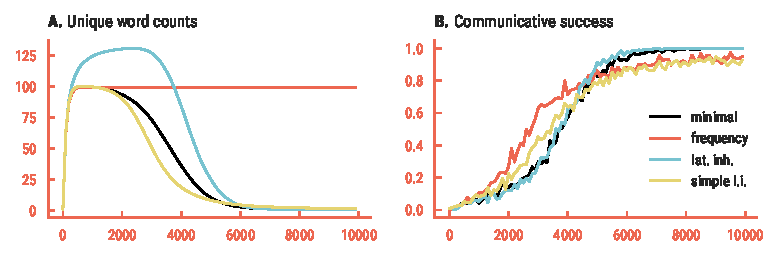
\includegraphics[trim=0.94cm 0 0 \figtopmargin]{LING01-results}
%	\caption{Comparison of the four strategies in table \ref{table:li-strategies}. Only the unique word count $N_{\text{unique}}(t)$ and communicative success $p_s(t)$ are shown.
%		\\[1em]
%		Results shown for 300 runs; $N=200$.
%		\label{fig:strategies}}
%\end{SCfigure}
%
%
%%Even when keeping $\delta_{\text{dec}} = s_{\text{min}} = 0$ fixed, a large portion of the parameter space remains unexplored and is marked as ‘intermediate strategies’.
%%We can say a bit more about this.
%%Note that scaling $\theta$ does not change the behaviour of the games; only the ratios between the paramaters matter.\footnote{\textcite{Wellens2012} discusses the effects of individual parameters, but this might not be the most sensible thing to do.}
%%More formally, let
%%\[
%%	\rho = \frac{\delta_{\text{inc}}}{\delta_{\text{inh}}}
%%\]
%%to be the ratio between the size of the increments and inhibition.
%%When $\rho \to 0$, that is, when inhibition is much stronger than the increments, the game starts to resemble the minimal naming game.
%%Conversely, when $\rho \to \infty$ one approaches the frequency strategy.
%
%
%\begin{SCtable}\sffamily\footnotesize\color{main}
%	\begin{tabular}{@{}lllllll@{}}
%		\toprule
%		&$\delta_{\text{init}}$	
%		& $\delta_{\text{inc}}$ 
%		&$\delta_{\text{inh}}$ 
%		&$\delta_{\text{dec}}$ 
%		&$s_{\text{min}}$ 
%		&$s_{\text{max}}$\\\midrule
%		\textsc{minimal strategy}		&1	&0	&1	&0	&0 	&$1$\\
%		\textsc{current strategy}		&1	&1	&1	&0	&0 	&$\infty$\\
%		\textsc{lateral inh.\ strategy}	&0.5	&0.1	&0.2	&0.2	&0	&$1$\\
%		\textsc{frequency strategy}		&1	&1	&0	&0	&0	&$\infty$\\
%		\bottomrule	
%	\end{tabular}
%	\caption{Parameter settings for various strategies. Note that equivalent parametrizations also exist; see main text.
%		\label{table:li-strategies}}
%\end{SCtable}
%
%%\begin{SCtable}\sffamily\footnotesize\color{main}
%%	\begin{tabular}{@{}lllllll@{}}
%%		\toprule
%%		&$\delta_{\text{init}}$	
%%		& $\delta_{\text{inc}}$ 
%%		&$\delta_{\text{inh}}$ 
%%		&$\delta_{\text{dec}}$ 
%%		&$s_{\text{min}}$ 
%%		&$s_{\text{max}}$\\\midrule
%%%		\textsc{degenerate strategy}	&$\alpha$	&0	&0	&0	&0 	&$\ge \alpha$\\
%%		\textsc{weak minimal strategy}	&$\alpha$	&$0$	&$<\alpha$	&$0$	&$0$ 	&$\ge \alpha$\\
%%		\textsc{minimal strategy}	&$\alpha$	&$0$	&$\ge\alpha$	&$0$	&$0$ 	&$\ge \alpha$\\
%%%			\textsc{minimal strategy}	&$\alpha$	&$>0$	&$\ge\alpha$	&$0$	&$0$ 	&$\alpha$\\
%%%		\textsc{approx. minimal strategy}	&$\alpha$	&$\beta$	&$>>\alpha+\beta$	&0	&0 	&$\ge \alpha$\\
%%		\textsc{intermediate strategies}	&$\alpha$	&$>0$	&$>0$	&$0$	&$0$ 	&$\infty$\\
%%	%	\textsc{li} strategy	&1	&1	&1	&0	&0 	&$\infty$\\
%%		\textsc{frequency strategy}	&$\alpha$	&$>0$	&$0$		&$0$		&$0$	&$\infty$\\
%%		\bottomrule	
%%	\end{tabular}
%%	\caption{Parameter settings of the \textsc{li}-game corresponding to various games
%%		\label{table:li-strategies}}
%%\end{SCtable}
%
%%Note that scaling $\theta$ results in the same behaviour, so the ratios between the parameters determine the behaviour of the model.\footnote{\textcite{Wellens2012} discusses the effects of individual parameters, which seems less informative.}
%
%\mcomment{Perhaps include the comments on the lateral inhibition strategy from \textcite{Steels2011}}


\section{Negotiating simple numerals}

As we have seen, the naming game can be adapted to get models of the standardization of bases (the base games),
but a more direct use of the naming games suggests itself: modelling the emergence of simple numerals.
Recall that both \textcite{VonMengden2008} and \textcite{Hurford1987} assumed that at some point words for the basic numerals had become available to the population.
Can the naming game capture the negotiation of \emph{multiple} words for all simple numerals simultaneously?

\subsection{The Number Naming Game}
Yes, it can. 
In fact, the very first naming games already concerned multiple ‘objects’.
The scenario was simplified after it was recognized that multiple objects often form an unnecessary complication \parencite{Wellens2012}. 
To see why this is the case, consider a \textsc{li}-naming game with a set of $L$ objects.
The population will have to negotiate an object--word mapping, that is, a object--word pair $(o, w)$ for every object $o$.
Every agent associates a score $s(o,w)$ to every pair.
The script of this game holds few surprises:


\begin{enumerate}
	\item A speaker $S$ and hearer $H$ are randomly selected from the population.
	\item The speaker randomly picks first an object $o$ from $\{o_1, \dots, o_L\}$ and second one of the associated words $w$ (generating one if it knows none).
	\item The hearer receives the pair $(o, w)$. Two things can happen:
		\begin{enumerate}
			\item The hearer knows the pair and communication is successful. Both agents update $s(o,w)$ by $\delta_{\text{inc}}$ and inhibit competing pairs $(o', w')$ with either $w' = w$ \emph{or} $o' = o$ by $\delta_{\text{inh}}$.
			\item The hearer does not know the pair and communication fails. The hearer adds the pair to its lexicon with score $\delta_{\text{init}}$ and the speaker discounts $s(o,w)$ by $\delta_{\text{dec}}$.
		\end{enumerate}
\end{enumerate}
%
The $(o,w)$-pairs thus take the role of words in the minimal naming game.

Now suppose that no word ever names two objects, that is, suppose there is no homonymy.
That means that whenever the hearer knows $w$, it necessarily knows the object $o$ it names.
So in the absence of homonymy, the agents are playing $L$ \emph{independent} \textsc{ng}'s simultaneously, one for every object \parencite{Baronchelli2008}.
As a result, the dynamics remain essentially the same.
Concretely, if $N_{\text{unique}}(t \mid o)$ is the unique number of words for object $o$ used in the population at time $t$; and $N_{\text{unique}}(t)$ is the number of unique $(o, w)$ pairs at time $t$, then 
\[
	N_{\text{unique}}(t) 
		= \sum_{o} N_{\text{unique}}(t \mid o) 
		= L \cdot N_{\text{unique}}(t \mid o_1).
\]
This is illustrated in figure \ref{fig:multi-word-minimal-naming-game}, which shows both $N_{\text{unique}}(t \mid o)$ for each $o$ (dashed) and $N_{\text{unique}}(t)$ (solid). 
It also shows that the time to convergence is multiplied by a factor $L$, as is to be expected when $L$ games are played simultaneously.
In short, the multi-object \textsc{ng} is fully determined by $L$ and the dynamics of the single-word \textsc{ng}%
	\footnote{More precisely, if $N_1(t)$ is some statistic of the single-word minimal \textsc{ng}, then the $L$-word minimal \textsc{ng} has statistic $N_L(t) = L \cdot N_1(t/L)$.}
— in the absence of homonymy. 
The latter is guaranteed whenever a newly generated word is actually \emph{new}.\footnote{Step 3a of the script then contains a redundancy; competing pairs with $w=w'$ and $o \neq o’$ cannot exist. In the presence of homonymy, however, this clause \emph{is} crucial.}

\begin{SCfigure}
	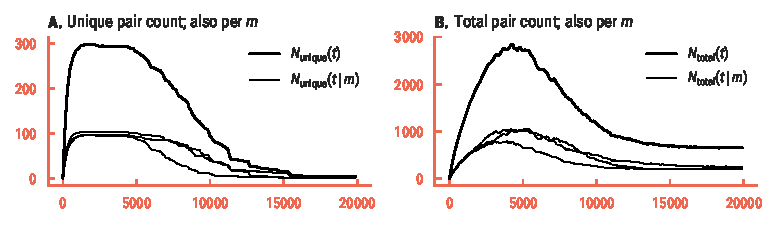
\includegraphics[trim=0.94cm 0 0 \figtopmargin]{FIG07-mw-naming-game}
	\caption{The multi-object \textsc{ng} (with $L=3$ objects) is the sum of independent single-word \textsc{ng}'s.
		Dashed lines show the statistics per object; solid lines for all $(o, w)$-pairs.
		The solid lines are the sums of the dashed lines.
		\\[1em]
		Results shown for 1 run; $N=200$, using the current strategy.
		\label{fig:multi-word-minimal-naming-game}}
\end{SCfigure}


\paragraph{Number Naming Game}
The lateral-inhibition naming game using the ‘current’ strategy ($\delta_{\text{inc}} = \delta_{\text{inh}} = \delta_{\text{init}} = 1$ and $\delta_{\text{dec}}=0$) to name $L>0$ objects — that I will call the \emph{Number Naming Game}.
When one takes the objects to be numbers, the game models the emergence of simple numerals. 
There is no need to further comment on the dynamics of this game; these are known from the above discussion.

%
%\paragraph{number-naming game}
%In my first experiments with the multi-word \textsc{ng}, homonymy \emph{did} occur.
%To cope with that, I adopted a lateral inhibition strategy.%
%	\footnote{This is an alternative fact. I was initially only aware of minimal strategies and extended those. Later my extension turned out to be known as a \textsc{li} strategy.}
%All further simulations will use this strategy, even though they homonymy does not occur.
%\mcomment{Ideally, I would probably change the strategy to be consistent with the literature, but that would mean rerunning all experiments...}
%Let $s(o, w)$ denote the score of the given pair.
%The update step (3) is changed as follows: 
%\begin{enumerate}\setcounter{enumi}{1}
%	\item The speaker randomly picks an object $o$ from $\{o_1, \dots, o_L\}$ and then randomly picks one of the words $w$ with $s(o,w) > 0$.
%	\item The hearer receives the pair $(o, w)$. Two things can happen:
%		\begin{enumerate}
%			\item The hearer knows the pair (success). Both agents increase $s(o, w)$ by $\delta_{\text{inc}}$ and decrease the score of (1) all $(o, w')$ with $w' \neq w$ and (2) all $(o', w)$ with $o' \neq o$ by $\delta_{\text{inh}}$.
%			\item The hearer does not know the pair (failure). The hearer adds the pair to its lexicon with score $s(o, w) = \delta_{\text{init}}$. The speaker decreases $s(o,w)$ by $\delta_{\text{decr}}$.
%		\end{enumerate}
%\end{enumerate}
%Here, we use $\delta_{\text{inc}} = \delta_{\text{inh}} = \delta_{\text{init}} = 1$ and $\delta_{\text{dec}} = 0$.



\subsection{The Counting Games}

As a model of the emergence of simple numerals, the Number \textsc{ng} has two closely related shortcomings: the lack of order and the possibility of gaps.
Although the order of the semantics carries over on the conventionalized set of simple numerals, nothing particular about the words suggests an order. %; order plays no role in the game.
It is therefore perfectly possible that an agent learns the word for 6 before it knows 4, resulting in a gappy numeral system.
That is odd: order and continuity are of crucial importance in numeral systems.



One might argue that the number-naming games embody a specific conception of number.
\textcite{Hurford1987} discerns three broad explanations of the continuity of the counting sequence.
In extreme form, the \emph{referential-pragmatic hypothesis} holds that cardinalities are properties of collections (‘threeness’) that are fairly directly perceptible — \emph{subitized}.
Continuity follows from the claim that $n$ is more likely to be expressed than $n+1$. 
The \emph{conceptual-verbal hypothesis}, in a Fodorian fashion, assumes we are born with the concepts \textsc{one}, \textsc{number} and \textsc{successor}.
Consequently, children cannot but construct a continuous sequence, like “little Peano’s.”
The \emph{ritual hypothesis}, finally, assumes numbers are the result of reciting a ritualized sequence; the meaning is grounded in the ritual of counting.
Prima facie, all of these positions are highly problematic and Hurford therefore suggests a synthesis: small numbers up to 3--4 are subitized and we learn the notion of successor only after exposure to a conventional counting sequence.

The number naming game corresponds to the \emph{referential-pragmatic hypothesis}.
We explicitly replaced objects by numbers — it can hardly get more referential. 
The goal of this section is to modify the number naming game in such a way that it more closely conforms to Hurford's synthesis.
I will do so by introducing three \emph{counting games} where agents conventionalize a \emph{counting sequence}.
That is a sequence of words (numerals), whose meaning is implicitly defined by their position in the sequence: the fifth word has the meaning 5 precisely because it is the fifth in the sequence.
Consequently, continuity and order become necessary properties, as some argue they should be \parencite{VonMengden2008}.


\paragraph{pairs and sequences}
In the number naming game, agents negotiated a set of $(o, w)$ pairs. 
We adapt this mechanism to negotiate a sequence described by pairs of consecutive numbers: $(\text{one}, \text{two}), (\text{two}, \text{three})$, and so on. 
%In the Counting Game, agent record the frequencies of such pairs of consecutive words.
%In this way they learn which words could follow a certain word.
To illustrate this, suppose an agent knows the following pairs:
\begin{align*}
	(\textsc{start}, \text{one}), 
	(\textsc{start}, \text{two}), 
	(\text{two}, \text{three}),
	(\text{two}, \text{four}),
	(\text{one}, \text{two}),
\end{align*}
where \textsc{start} indicates the start of the counting sequence. The agent can form the following sequences:
\begin{align*}
	&\text{\textsc{start}, one, two, three},
	&&\text{\textsc{start}, one, two, four},\\
	&\text{\textsc{start}, two, three},
	&&\text{\textsc{start}, two, four}
\end{align*}
Other agents might be able to form different sequences, but the idea is that after many interactions, a consensus will emerge where only one sequence remains possible.
Of course, in every round agents will now communicate a set of words. 
This generalizes the naming game where agents only exchanged a single word.
%The precise script varies slightly in the three games I present below.




\begin{SCfigure}
	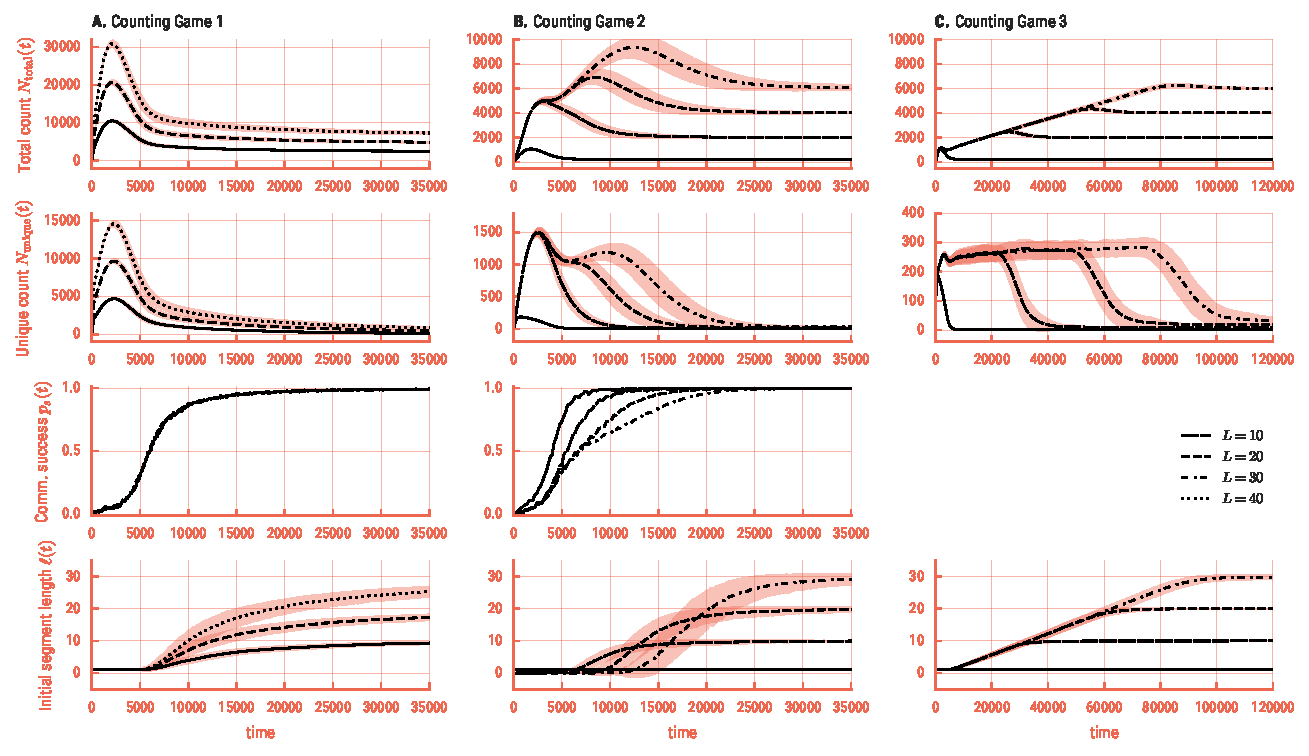
\includegraphics[trim=0 0 0.61cm 0,angle=90,origin=c]{all-counting-games}
	\caption{Detailed comparison of the dynamics of all three counting games. 
		If you rotate the page, every column (A, B, and C) correspond to a game. In every row you find the same statistics for all games: the total counts $N_{\text{total}}(t)$, the unique counts $N_{\text{unique}}$, communiative success $p_s(t)$ and the $\ell(t)$, the length of the counting sequence about which agreement has been reached.
		\\[1em]
		Results shown for $N=200$; avg.\ of 600 runs, 1 std.\ shaded.
		\label{fig:all-counting-games}}
\end{SCfigure}



\paragraph{Counting Game 1}
The first counting game uses the following script.
\begin{enumerate}
	\item A speaker $S$ and hearer $H$ are randomly selected.
	\item The speaker counts to a random number $n \le L$. 
	\item Starting from $w_0 = \textsc{start}$, the speker iteratively chooses the next pair $(w_i, w_{i+1})$ with the highest score, generating new pairs if necessary. It then concatenates the pairs to form a sequence $(\textsc{start}, w_1, w_2, \dots, w_L)$. 
	\item The hearer receives the sequence and for every pair $(w_i, w_{i+1})$ updates the scores as in the Number Naming Game.
\end{enumerate}
Counting Game 1 is thus a naming game when $L=1$.

To assess the convergence of the counting games use another statistic, the \emph{initial segment length} $\ell(t)$ which is the length of initial segment of the counting sequence about which the entire population agrees at time $t$.
An additional complication arises when pairs are inhibited and removed:  lexica become polluted with unusable words. 
If one thinks of the pairs as describing a tree with \textsc{start} at the root, the loss of a single pair can render an entire branch inaccessible.
To keep statistics like $N_{\text{total}}$ informative, all inaccessible pairs are removed before collecting the statistics.
Finally, the communicative succes is no longer boolean but averaged over all words in a round.
If an agent knows $4$ of the $5$ pairs, we estimate $p_s(t) = 0.8$.


The behaviour of counting game 1 is shown in figure \ref{fig:all-counting-games}A for three values of $L$, next to the other counting games we discuss later.
First of all, the population over time settles on a fixed sequence of length $L=10, 20$ or $30$.
However, the characteristic difference between $N_{\text{total}}$ and $N_{\text{unique}}$ seems to have disappeared.
$N_{\text{total}}$ grows up to around $1000 L$; $N_{\text{unique}}(t)$ peaks around roughly the same time at $500 L$.
Most striking is the communicative success $p_s(t)$, which does not seem to depend on $L$.
Agents thus learn to count to $L$ equally quickly for any $L$.
That is reflected in $\ell(t)$.
It shows that the further the population has to count, the faster they agree about an initial segment. 
How can that be?
%Formally, if $t_L(n)$ is the time at which agents counting to $L$ agree about the first $n$ numbers, i.e.\  that $\ell(t_L) = n$, then $t_{10}(n) > t_{20}(n) > t_{30}(n)$.


My implementation happens to represent words by successive integers (rather than strings). 
As a result, successively generated words can easily be recognized. 
It turns out that the counting sequence adopted by the population often consists of (fragments of) smaller sequences generated by a single agent.
For example, one might find a sequence of the form
\[
	\textsc{start}, \;
	\underbrace{212, 213, 214}_{\text{fragment 1}}, \; 
	\underbrace{350, 351, 352, 353}_{\text{fragment 2}}, \;
	\underbrace{658, 659, 660}_{\text{fragment 3}}.
\]
Again, the numbers are ‘words’.
To estimate how common this is, I computed the number of such fragments in the final counting sequence in all 600 simulation runs.\footnote{
	In some runs, not all agents had agreed on the same sequence in the final round.
	In those cases I used the most frequent sequence, and ignored all runs where the most frequent sequence was used by less than 50\% of the population.%
	For $L=0$, the most frequent sequence after 150 000 rounds was adopted by less than half the population in 0 out of 600 runs; for $L=20$ in 10 out of 600; and for $L=30$ in 130 out of 600 runs. These I ignored.}
A histogram of the result is shown in figure \ref{fig:counting-game-I-num-groups}. %todo
When the number of fragments is 1, a single agent generated the final sequence; and when it is close to $L$, every word is generated by a different agent.
Also note that if two sequences of length $L=10$ and $L=30$ both consist of four fragments, these will on average be much longer for $L=30$ (7.5 rather than 2.5 words).

These results suggest that population adapts to a higher $L$ by exchanging \emph{fragments} rather than pairs.
Since it moreover uses larger fragments for larger $L$, convergence times remain approximately stable. 
Fascinating as this may be, it presents a problem for numeral systems, where the use of fragments seems unwarranted. 
The next game circumvents that.


\begin{SCfigure}
	% Computed in Counting Game I notebook; exp01
	\hspace{-1.25cm}
	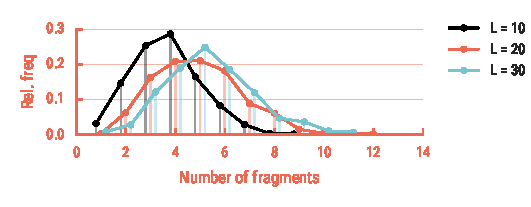
\includegraphics{counting-game-I-num-groups}
	\caption{The number of ‘fragments’ in the final counting sequence across 600 simulation runs. Each fragment is a sequence of words successively generated by a single agent. 
		\label{fig:counting-game-I-num-groups}}
\end{SCfigure}

\mcomment{Maybe leave out game 2 altogether? I don’t really have anything to say about it, other than that the dynamics are funny}


\paragraph{Counting Game 2}
In Counting Game 2, in every round an agent can invent at most one new pair, whose score remains 0. 
Moreover, they do not count to a random number $n \in \{0, \dots, L\}$ but count as far as they get, but up to $L$.
Agents can thus only adopt a new pair if \emph{another agent taught them} how to count on.
These relatively minor changes have substantial effects on the dynamics, as shown in figure \ref{fig:all-counting-games}B.


Several things should be noted.
First, both $N_{\text{unique}}$ and $N_{\text{total}}$ have two local maxima for $L>10$. 
The first happens around the same time as in counting game 1.
The maximum of $N_{\text{unique}}$ is the same for all $L$.
Communicative success $p_s(t)$ now does depend on $L$; it takes the population longer to reach high $p_s(t)$ if $L = 30$.
Finally, the emerging counting sequences hardly contain any fragments.

[...]



\paragraph{(Joint) Counting Game 3}
The third counting game brings further changes to the script: the speaker no longer counts alone, but \emph{jointly} with the hearer.
Starting with \textsc{start}, the speaker utters the first word. 
Both agents perform the usual updates, but \emph{only if the hearer knows the word}, i.e.\ if communication was successful, they continue with the next word.
They continue as long as communication does not break down, until they reach $L$.
Since communicative success $p_s(t)$ is in not very informative in this game, it is not shown in figure \ref{fig:all-counting-games}C.
But what we do see is that the convergence time appears to scale linearly with $L$. 
That is, learning to count to 20 takes twice as long as counting to 10.
However, convergence takes much longer.


\mcomment{To do: write up interpretation of results; maybe discuss with Jelle first}


\end{document}



\paragraph{Counting Game I}


Adding a base. 
In Hurfords second account, bases result from the grouping of objects.
We wish to reflect the grouping in the model.
Suppose every agent keeps track of which possible group sizes it could use.
On every interaction, it picks a group size and arranges the objects in groups of the desired size. 
It then communicates the group size, the number of groups and how many items are ungrouped. 
This corresponds to decomposing the number as $n = f \times b + r$ with $b$ the base or group size, $f$ the number of groups and $r$ the remainder.
Since numbers are communicated as sequences, similarly to the simple Counting Game, the hearer can learn both the counting sequence and a base at the same time.
Such a game would thus be a mix of the counting game (to negotiate the sequences) and the naming game (to negotiate the value of the base). 

I experimented with such a game and there are two important problems. 
The first is that negotiating a base value is much simpler than negotiating a sequence; it really amounts to negotiating a single value, rather than a sequence of word pairs.
The population thus very quickly settles on a base, mostly before the agents even agree about the first counting term.
The resulting bases are moreover low (mostly 2 and 3)




\section{Emergent numeral systems?}

The idea most clearly formulated by \textcite{Hurford2007} was that numeral systems emerge from a practice of counting.
People encounter a collection of objects and start counting them off relying on some fixed sequence.
But at some point, the sequence ends and they group all the items encountered so far.
They continue by counting off the remaining items, until they reach the limit of the counting sequence, and so on, and so on.
This hypothetically leads to expressions such as \lng{five tens and four} and gives rise to bases.

This account assumes that a counting sequence exists before a the bases emerge. 
Indeed, the group size is completely determined by the length of the counting sequence.
All three counting games outlined above capture the negotiation of a counting sequence, but do not yet incorporate the grouping.


This, one might say, should be unproblematic: introduce an additional naming game to simultaneously negotiate the group size, the base.



% Print the bibliography
\showbibliography



\end{document}
